\chapter{Simulating Mode-Matching with FINESSE}
In Chapter 2, the optical gain from differential arm motion was determined analytically with very few approximations but in actuality, LIGO has more degrees of freedom which make precise calculations very cumbersome.  The complexity scales very rapidly in application to the main interferometer and mode matching is no exception so it is useful to use a full scale numerical simulation to extract as much information as possible.  FINESSE \cite{FinesseManual} \cite{FinesseTechniques} is one of the leading full-scale interferometer simulation tools which uses the linear input-output relations of electromagnetic fields to model optical properties of the LIGO interferometer.  This chapter uses FINESSE to model the quantum limited noise sensitivity with mode mismatch at key points in the interferometer and determine which actuators are needed for optimal matching into the output mode cleaner.  This is extremely important in the current generation of Advanced LIGO when squeezing is implemented because of the sensitivity to losses between the optical parametric oscillator and the interferometer cavities.  By using FINESSE's ability to incorporate higher order beams and RF sidebands, it is possible to quickly and accurately model mode matching.

\begin{figure}[ht!]
	\centering
	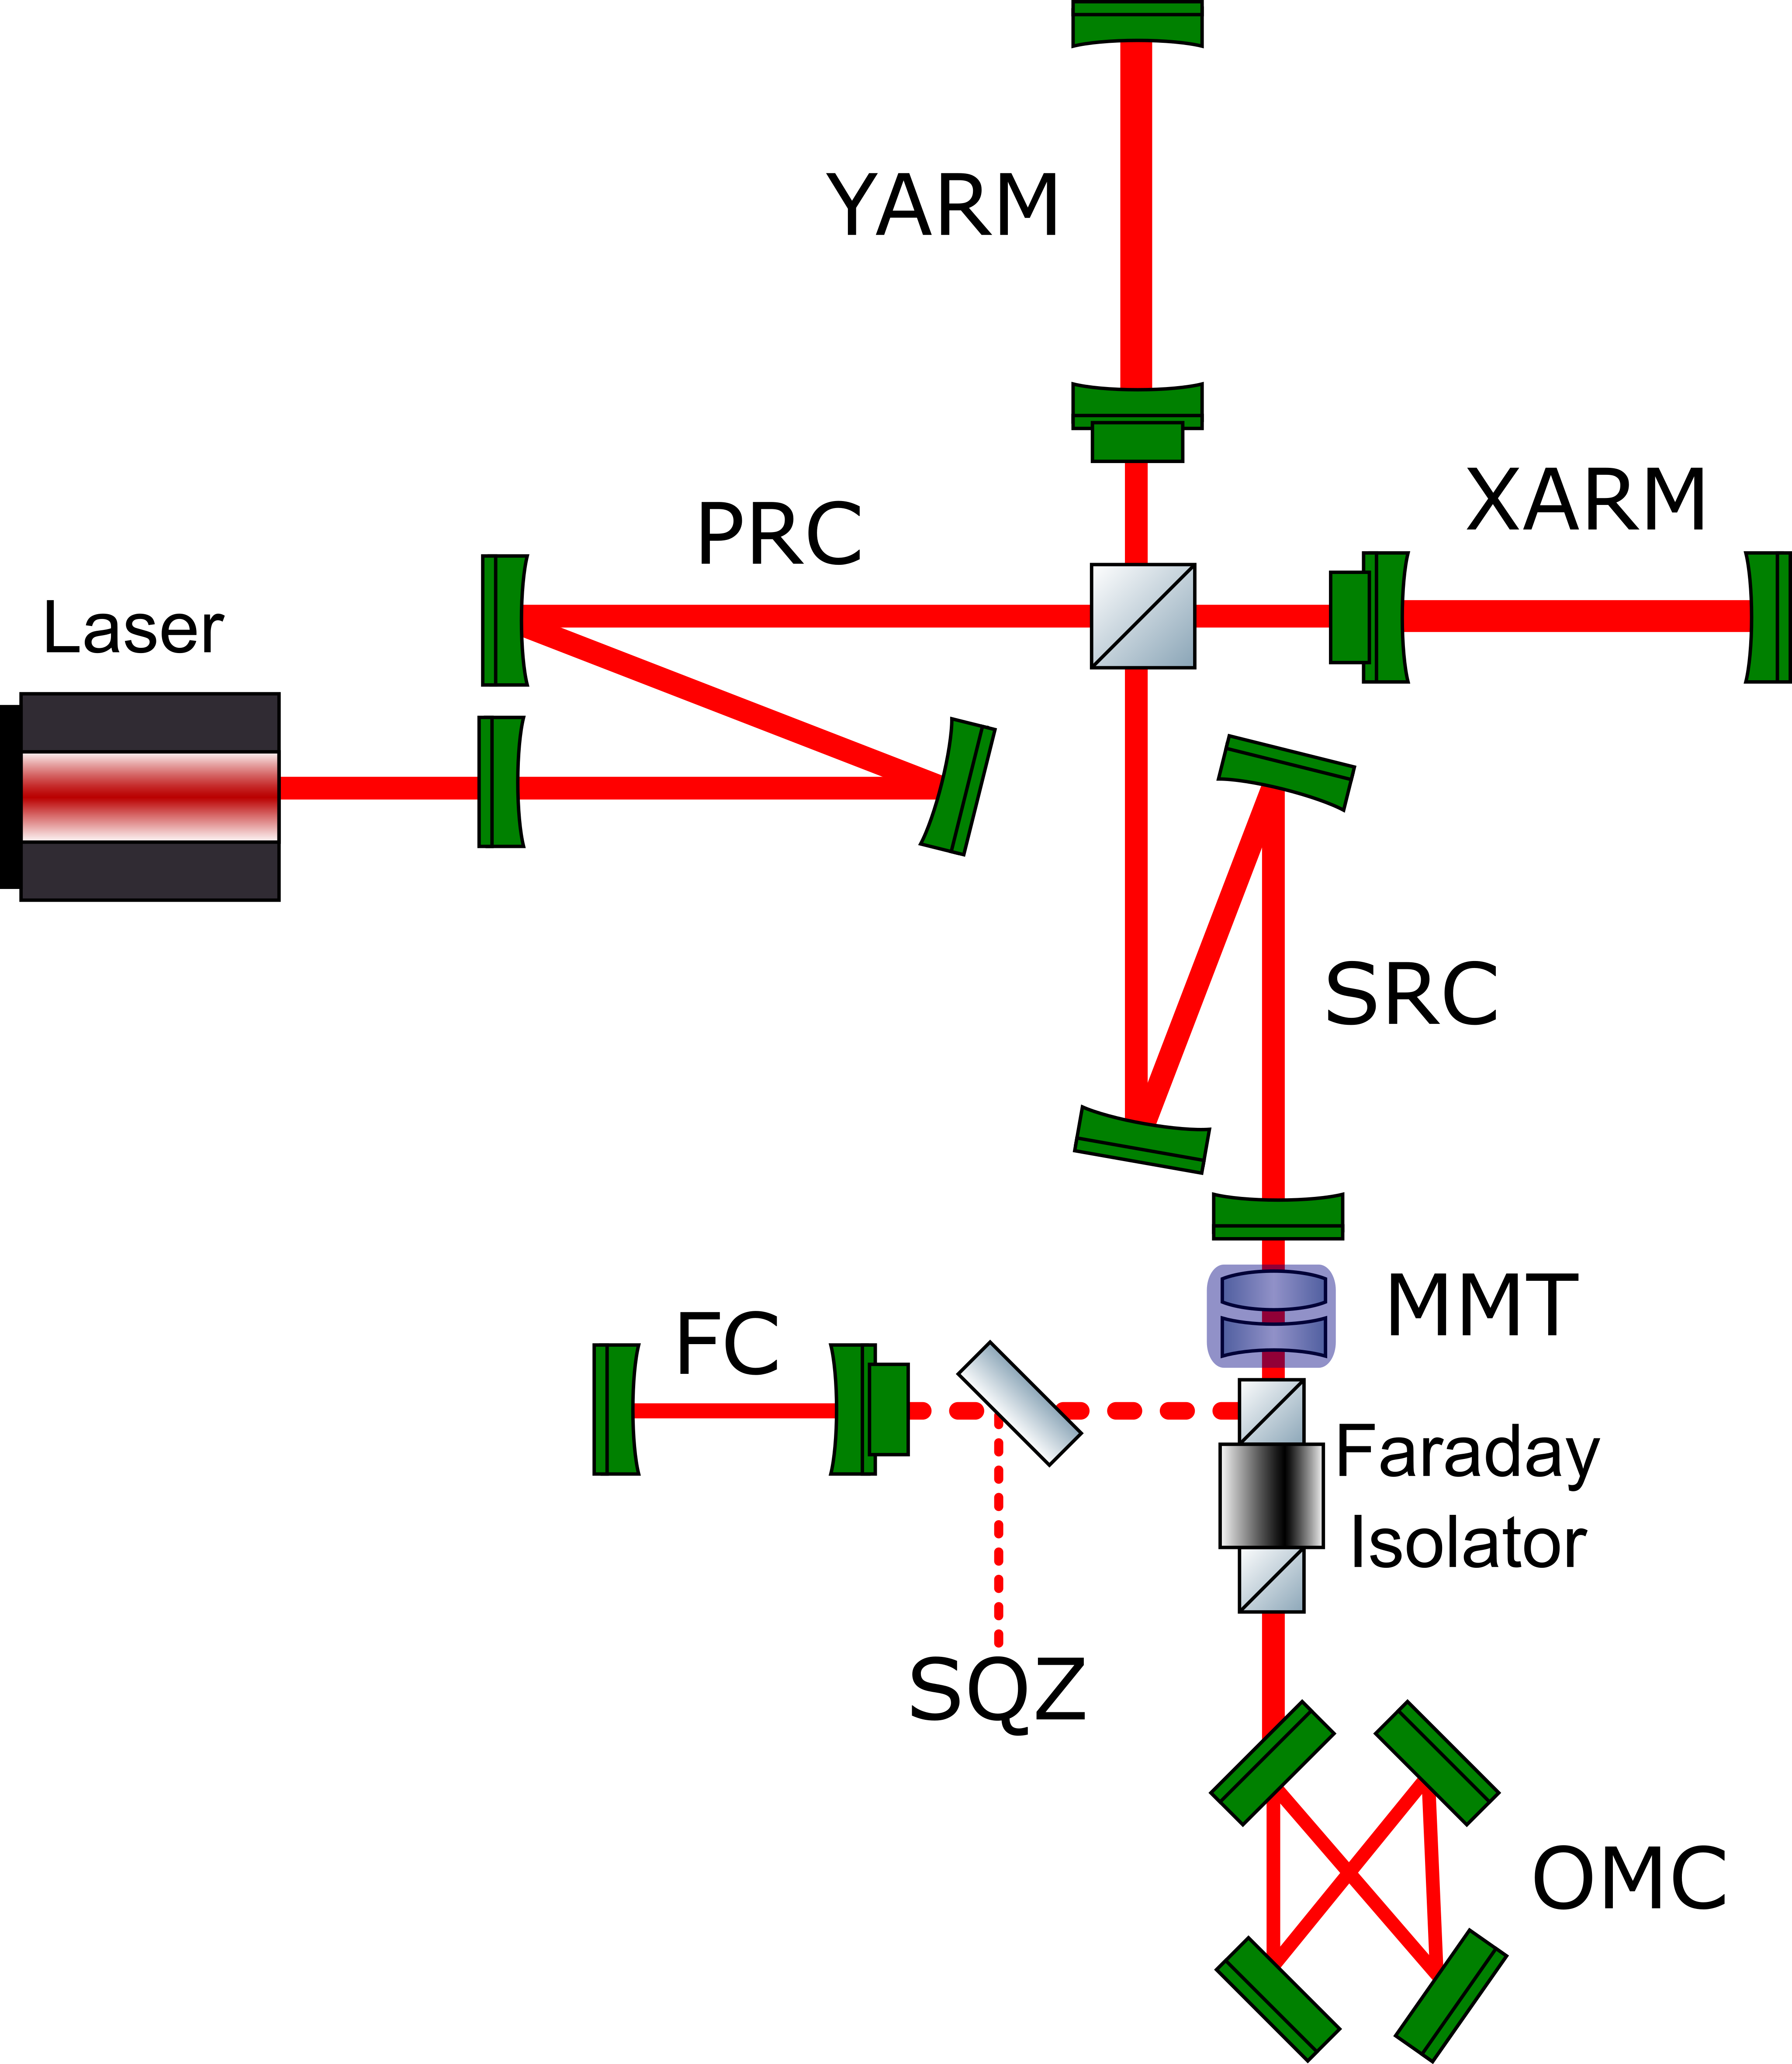
\includegraphics[width=0.8 \textwidth]{../Figures/FullIFO_FINESSE.png}
	\caption[Full interferometer simulation with FINESSE.]
	{\textbf{Full interferometer simulation with FINESSE.} 
		This includes squeezed light injection, a lossless 16-meter filter cavity, and an ideal mode matching telescope (highlighted in blue) at the signal recycling output port which can be turned on/off to determine the SRC mode mismatches without additional lensing effects when changing the radius of curvatures.  For brevity, the input mode cleaner is omitted in the schematic but is also a resonant cavity in the simulation where it is approximated to have small thermal effects and is at least 99.9\% mode matched to the interferometer.  Optical parameters are taken from the as-designed values for advanced LIGO and a few key variables are replaced with H1 specific constants.
	}
	\label{fig:IFO_FINESSE}
\end{figure}

	\section{FINESSE Simulations}
	The power of numerical simulations has an interesting dual advantage, firstly, optical parameters which are difficult to measure such as Gouy phase or higher order mode content can be directly calculated to guide in designing future systems. Secondly, when analytical calculations become unwieldy, numerical methods accurately describe complicated optical responses in the presence of perturbations or imperfections.
		
	\begin{figure}[h]
		\centering
		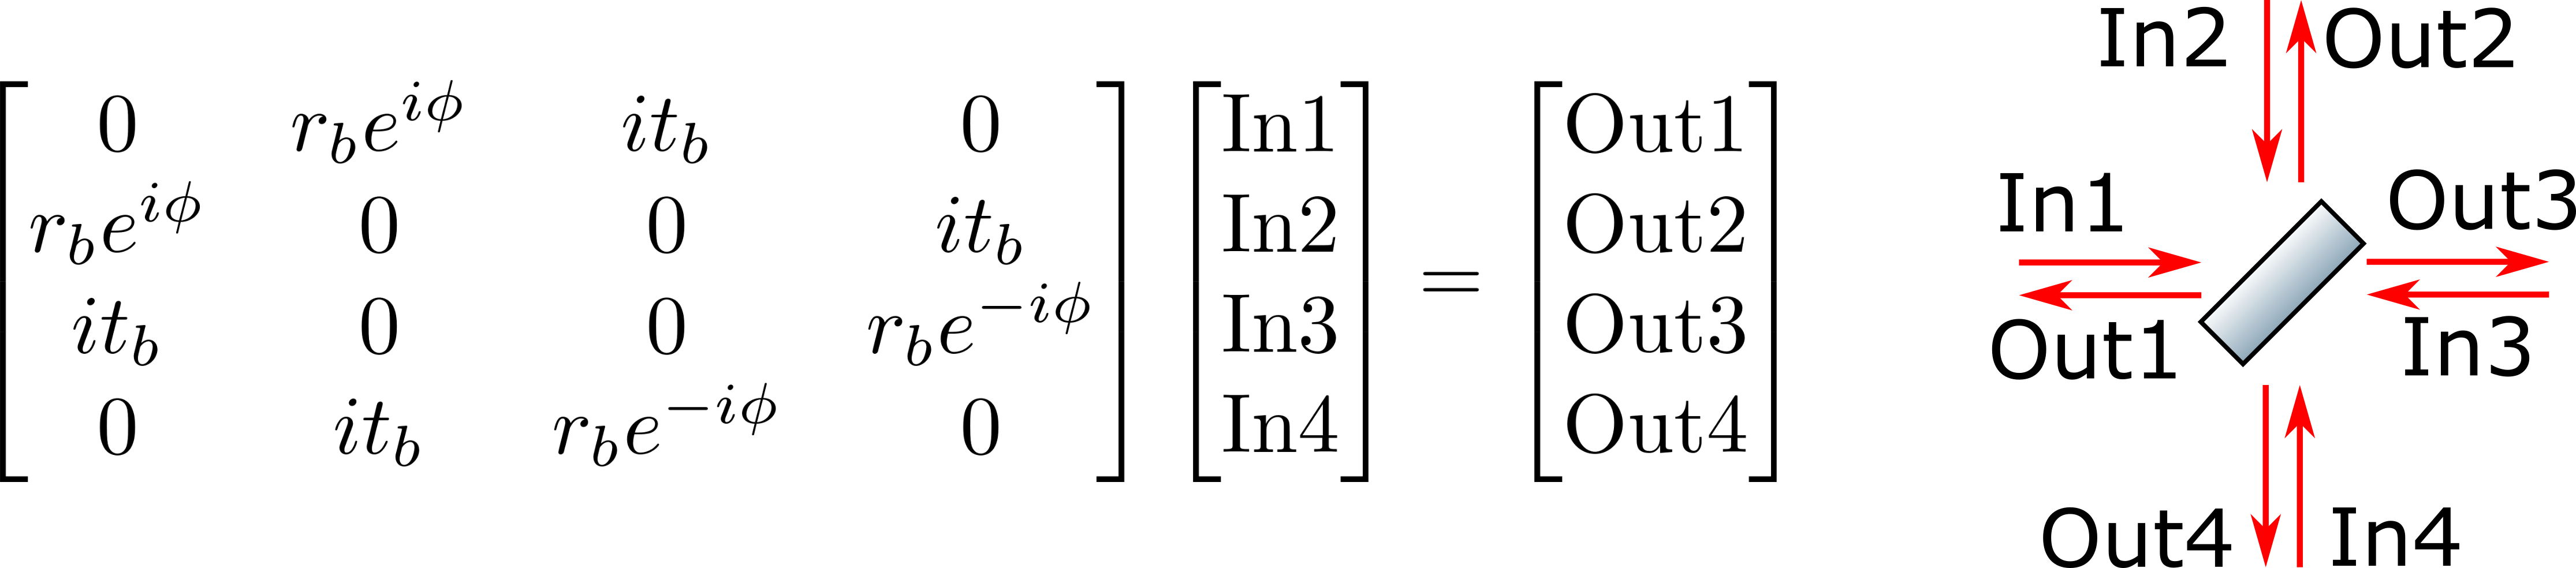
\includegraphics[width=0.8 \textwidth]{../Figures/bs_matrix_pic.png}
		\caption[How FINESSE sees a beamsplitter.]
		{\textbf{How FINESSE sees a beamsplitter.} 	An example of the coupling matrix for an arbitrary beamsplitter with reflectivity, $r_b$, and transmissivity, $t_b$. Another free parameter for a beamsplitter is the phase shift $\phi = 2 \phi_u \frac{\omega}{\omega_0} \cos(\alpha)$, where $\phi_u$ is a user defined phase that can be varied for a simulation (such as dithering), $\omega$/$\omega_0$ is the ratio of the reflected to incident angular wave frequency and $\alpha$ is the angle between the beamsplitter front surface and the incident field vector In1.  As it turns out, most of the resonators in the following simulations use beamsplitters to represent the cavity mirrors.
		}
		\label{fig:FINESSE_bs}
	\end{figure}

	An Advanced LIGO configuration file \cite{FinesseH1} which utilizes as-designed values for the lengths and optical parameters serves as a good starting point for simulating the entire interferometer.  To incorporate more realistic numbers, in-situ measurements were taken at Hanford with a beam scanner and ruler at HAM6 to understand the Gaussian beam shape entering the output mode cleaner. By defining the optical parameters and distances, FINESSE creates coupling matrices for individual components which are generally comprised of mirrors, spaces, or beamsplitters.  Some specialized components are also useful such as modulators to create sideband fields, Faraday isolators, and detectors (both amplitude and power).  For each component, there are corresponding nodes that link the entire optical system together.  The coupling matrices are compiled into an interferometer matrix and the solutions are solved numerically,
	\begin{equation}
	\hat{M}_{ij}^{\text{IFO}} \ket{x_{\text{sol}}} = \ket{x_{\text{input}}}
	\end{equation}
	where $\ket{x_{\text{sol}}}$ and $\ket{x_{\text{input}}}$ are the solution and input vectors, respectively. Generally, the right hand side is made up of laser inputs, modulator sidebands, noise, and signal sidebands. This form has incredible efficiency and can represent the entire interferometer in a single matrix with direct access to all field amplitudes.  In addition, changing optical parameters during a simulation is made easier by varying the coupling coefficients after the matrix has been calculated so the algorithm does not have to re-compute every term.
	\begin{figure}[t!]
		\centering
		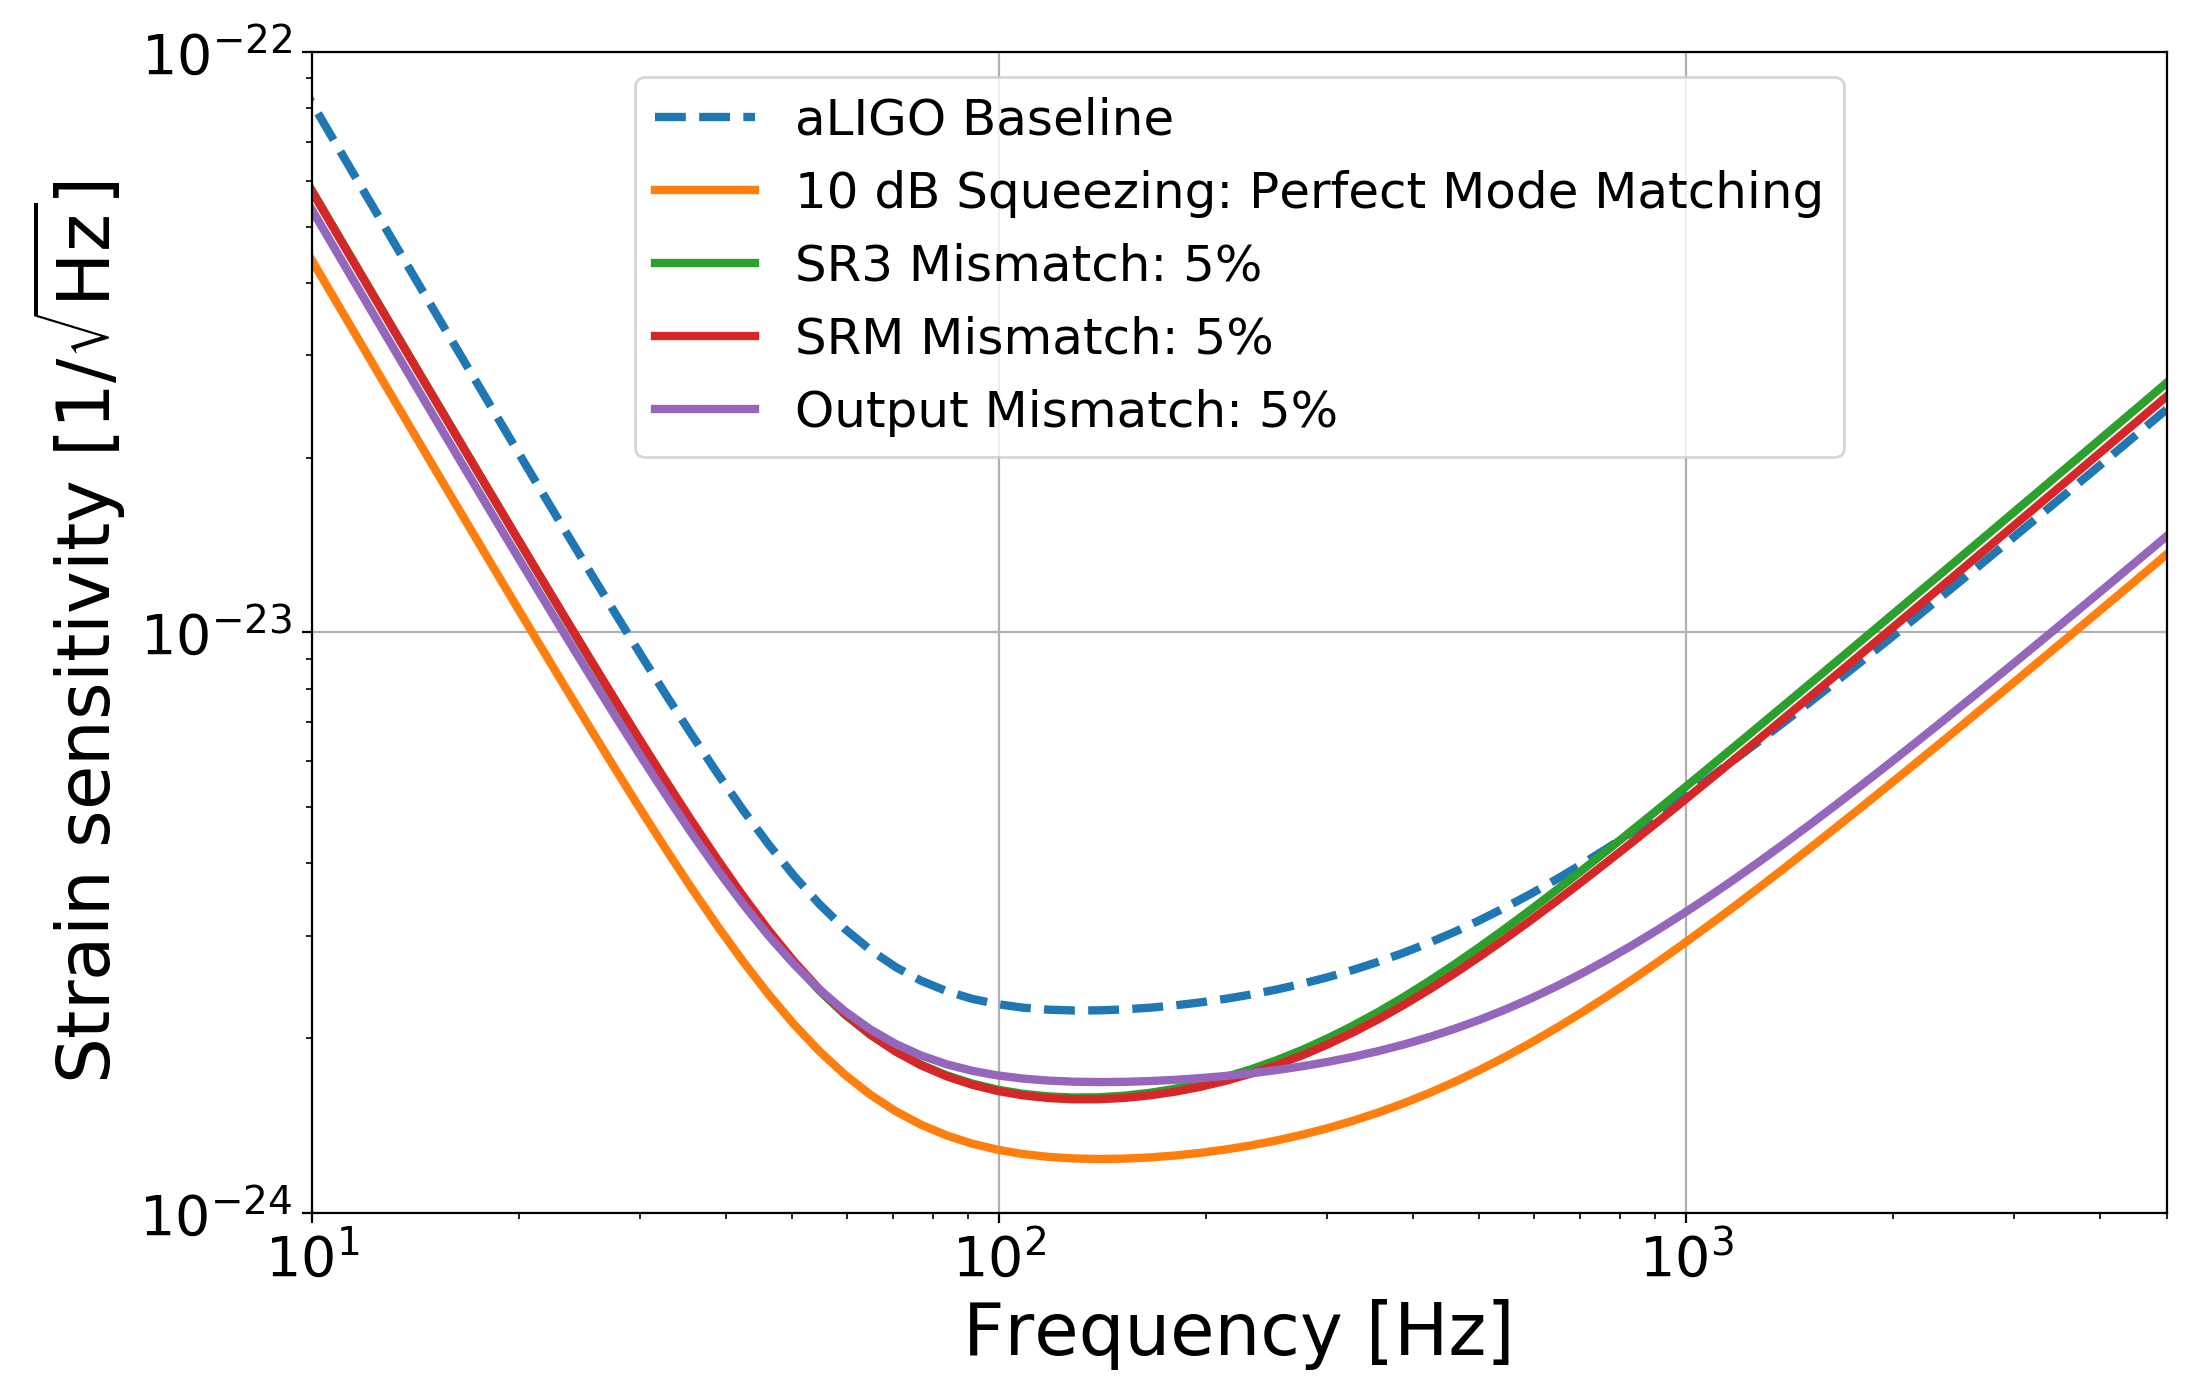
\includegraphics[width=1.0 \textwidth]{../Figures/QM_sens_compare_mismatches.png}
		\caption[Quantum limited sensitivity simulation to compare mismatches in the presence of squeezed light.]
		{\textbf{Quantum limited sensitivity simulation to compare mismatches in the presence of squeezed light.} 
			With 10 db of broadband squeezing, the simulation introduced mismatch at various actuators to change the mode shape at the output port.  Although there is still 5\% mismatch in each case, the introduction of quantum noise and the degradation of squeezing is much worse when introducing losses in the signal recycling cavity as opposed to the output train.  In addition, mismatching the signal recycling cavity will change the relative phase angle between the interferometer and squeezed light which has to be re-optimized.	
		}
		\label{fig:QM_lim_sens_mismatch}
	\end{figure}
	\section{Effects of Signal Recycling Mismatch}
	Beam tracing in FINESSE starts by determining the q-parameters for each user defined cavity. If there are multiple cavities, it will calculate in the order written and the last cavity in the parameter file sets the basis of populating the rest of the interferometer.  Table \ref{tbl:cav_params} shows the extracted cavity values for reference.  The algorithm continues by automatically propagating the laser beam through each node via ABCD transformation methods. For a perfectly mode-matched interferometer, the q's at each node are the same no matter which cavity basis is chosen but this is not true when introducing thermal lensing or errors for individual resonators.   At this point, it becomes extremely important to properly track the q-parameters because they are used to calculate the overall mismatch between cavities. To simplify the use of multiple coupled resonators, it is useful to turn all but one of the cavity commands off so that only one basis q-parameter is explicitly used and there is no ambiguity.  
	
	FINESSE has the ability to determine two parameters which calculate the sensitivity: noise and signal.  By default, vacuum fluctuations are present at each unused port and associated optical losses.  This methodology can be verified analytically using the full quantum mechanical description in Section \ref{Sec:QuantumNoise} and the semi-classical Schottky shot noise estimation.  For radiation pressure effects, the mechanical transfer function is defined by a simpled pendulum with $H(f) \propto \frac{1}{M \; f^2}$ dependence above the resonance frequency which is chosen to be approximately 0.1 Hz for these simulations.  As previously shown in Section \ref{Sec:QuantumNoise}, the radiation pressure effects are proportional to the input laser power and converts amplitude fluctuations into phase noise.  Naturally, this is a nonlinear equation so FINESSE makes certain approximations which reduces the complexity,
	\begin{enumerate}
		\item Induced motion from radiation pressure is very small compared to the light wavelength so the equations of motion can be linearized.
		\item Signal sideband frequencies are very small compared to the optical sidebands created by the modulator such that the carrier creates a much larger radiation pressure effect.
		\item The amplitude of signal sidebands are much smaller compared to the carrier.
	\end{enumerate}
	In terms of gravitational wave detectors, these approximations are reasonable because the machines tend to operate with closed-loop control systems and in steady-state equilibrium.  Also, the signal sidebands never reach above 8 kilohertz for two reasons: astrophysical sources from compact binaries coalesce at around 1.5 kHz and the Nyquist frequency for the differential arm channel is sampled at 16 kHz so the Nyquist frequency is much smaller compared to the 9 MHz sideband from the electro-optical modulator.  
	
	To generate the signal, differential arm motion is simulated by varying the two arm cavity lengths 180 degrees out of phase and measuring the optical gain transfer function at the output mode cleaner transmission port.  The results can be compared directly to the analytical transfer function described be equation \ref{eq:DRFP_opt_gain} to verify the right DC amplitude and pole frequency.  Figure \ref{fig:IFO_FINESSE} shows the results of mode mismatch affecting the quantum limited noise sensitivity.
	
	With regards to the squeezer implementation, the model applies both squeezed light and a filter cavity before entering the interferometer to compare the effect of mode-matching losses on the quantum limited sensitivity.  In FINESSE, the squeezer node employs classical sideband implementation while in reality, modified vacuum is generated using the optical parametric oscillator (OPO) which is a bow-tie cavity with a nonlinear optic that is not yet handled by the available FINESSE components and the nonlinear crystal actually keeps the cavity from being geometrically unstable. So for now, it is enough to use quantum noise sidebands with defined phase and amplitude variances have two open parameters, the squeezing gain and phase angle. 
	
	\begin{figure}[ht!]
		\centering
		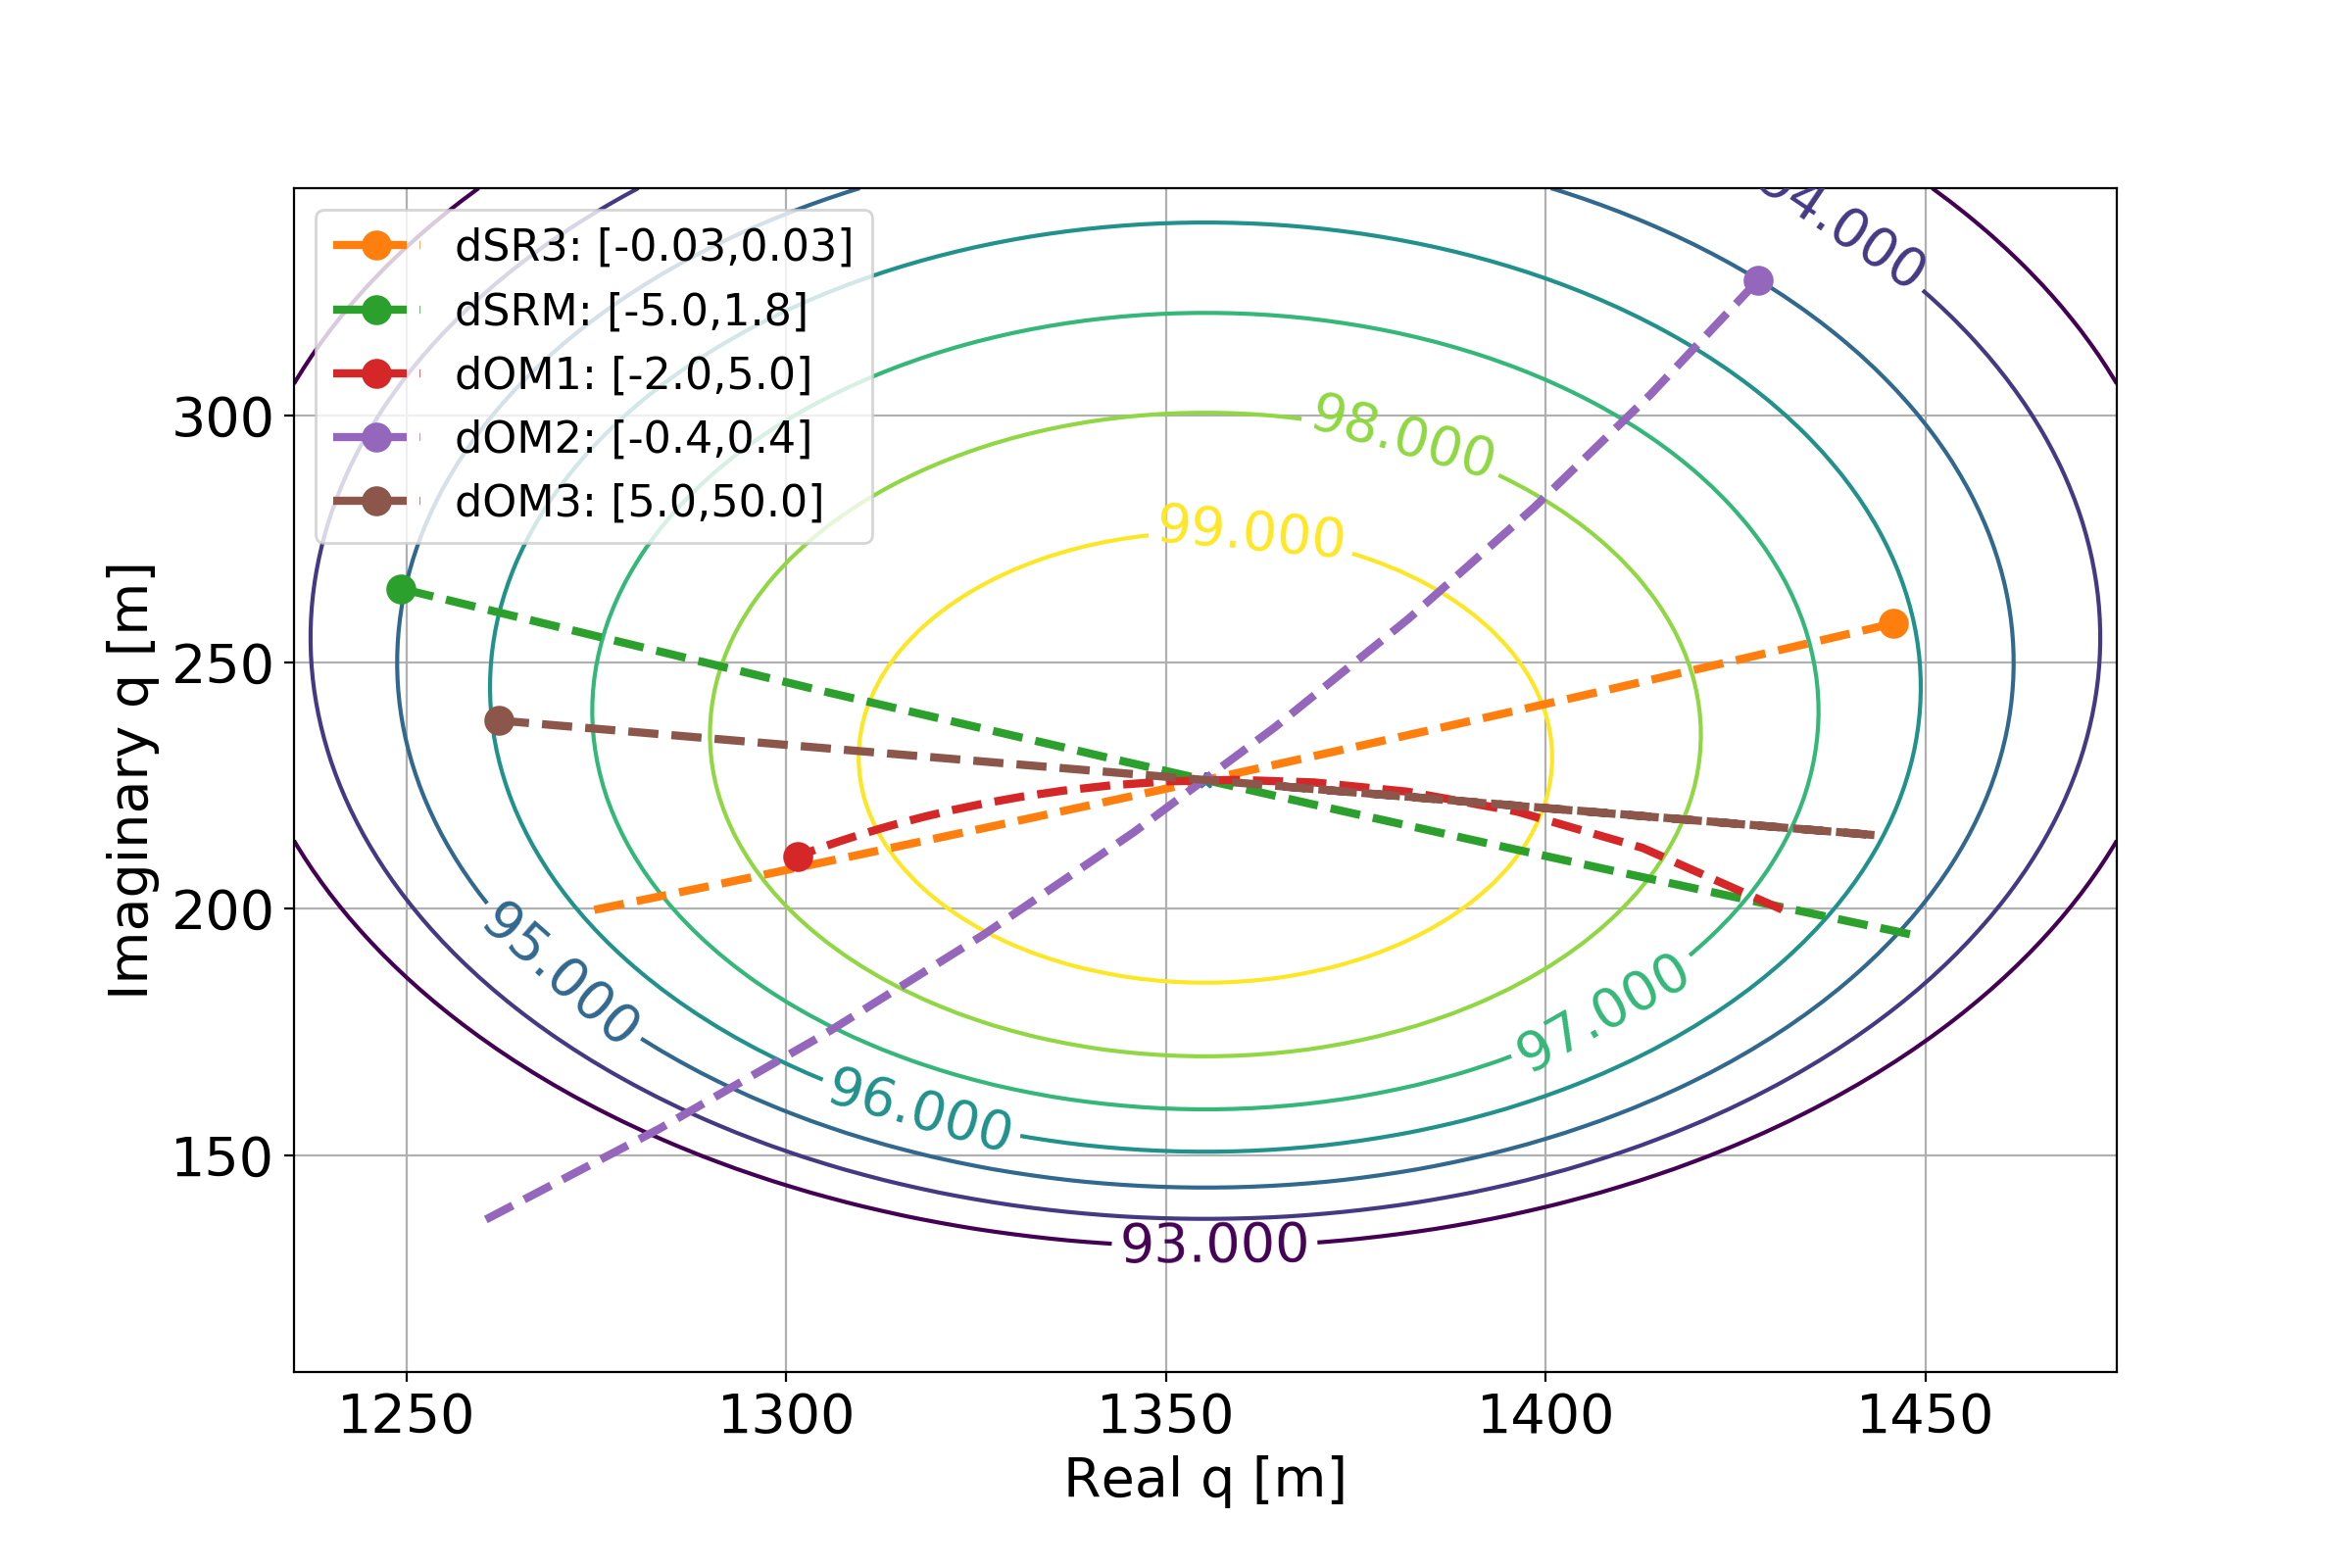
\includegraphics[width=0.9 \textwidth]{../Figures/OutputAct_Gouyphase.png}
		\caption[Simulating the output actuator phase spaces projected onto the OMC mode basis.]
		{\textbf{Simulating the output actuator phase spaces projected onto the OMC mode basis.} The ending dots indicate the positive direction for changing radii of curvature as seen by the various optics.  Also, the change in radii of curvature in units of meters is shown on the legend.
		}
		\label{fig:act_phase_space}
	\end{figure}
	
	LIGO's coupled optical cavities allow for a large parameter space when trying to match multiple resonators.   Changing the curvature of an optic in the signal recycling cavity will obviously change its overlap with the output mode cleaner but the effect will also vary the arm mode propagation to the OMC as well.  This will have a confusing result because it is impossible to discern whether the degradation in performance is due to the arm or SRC mismatch.  One of the ways to get around this is to implement a perfect mode-matching telescope between the SRC and OMC to keep the arm modes consistent with the output mode cleaner so that the only effect on the interferometer is a non-optimal signal recycling cavity.  The deterioration in sensitivity when mismatching the SRC has a two-fold effect, the introduction of vacuum fluctuations will degrade the squeezed field in a nonlinear fashion hence increasing the noise (even with perfect squeezing phase).  On top of that, extra SRC losses will affect the total optical signal gain at the antisymmetric port, which means sacrificing some losses in the SRC to mode match the squeezer field will not actually improve the sensitivity.  Comparatively, the extra losses introduced at the antisymmetric port before entering the output mode cleaner will only see increased losses that couple quantum vacuum.  The comparison is shown in Figure \ref{fig:QM_lim_sens_mismatch}.
	
	By allowing FINESSE to do the ray tracing algorithm for the entire interferometer, it is relatively straightforward to change the radii of curvature for different optics and project the effect onto the OMC in order to understand the orthogonality when choosing mirrors for mode matching.  In Figure \ref{fig:act_phase_space}, the most orthogonal actuators for small mismatches happen to be SRM and OM2, however, OM1 becomes quadratic much more quickly which leads to increased range. It is worthwhile to note that some literature will convert the phase space units to waist size and curvature instead of the imaginary and real parts of the q-parameter.
	
	A useful tool to understand the actuation matrix in a full interferometer configuration is to calculate the induced waist position or size shift per diopter in Figures \ref{tbl:x_act_matrix} and \ref{tbl:y_act_matrix}.  The code runs through each optic and slightly varies the radius of curvature or focal length and traces the beam for every cavity eigenmode.  This assumes the mismatches are relatively small so the slope is linear and can give a bit of insight on the directionality and magnitude of the actuators.

	\begin{sidewaystable}
	\centering
	\begin{tabular}{|l||r|r|r|r|r|r|r|r|}
		\hline
		{} &     PRC w &    PRC S &     SRC w &    SRC S &    ARMs w &   ARMs S &   OMC w &     OMC S \\
		\hline
		\hline
		PRM   &     4.537 &    0.006 &     0.000 &    0.000 &     0.000 &    0.000 &   0.000 &     0.000 \\
		PR2   &   -45.004 &   -0.058 &     0.000 &    0.000 &     0.000 &    0.000 &   0.000 &     0.000 \\
		PR3   & -3321.891 &   -4.315 &     0.000 &    0.000 &     0.000 &    0.000 &   0.000 &     0.000 \\
		SRM   &     0.000 &    0.000 &    -5.097 &   -0.006 &     0.000 &    0.000 &   0.875 &     1.114 \\
		SR2   &     0.000 &    0.000 &  -128.889 &   -0.160 &     0.000 &    0.000 &  -2.792 &   -99.513 \\
		SR3   &     0.000 &    0.000 & -5460.964 &   -6.774 &     0.000 &    0.000 & -19.564 & -4294.447 \\
		ITMTL & -3188.263 & 4142.666 & -5254.308 & 4140.289 &     0.000 & 	 0.000 &   0.000 &     0.000 \\
		ITM   & -2310.433 & 3002.047 & -3807.633 & 3000.325 & -1827.435 & 3002.782 &   0.000 &     0.000 \\
		ETM   &     0.000 &    0.000 &     0.000 &    0.000 &  3774.807 &    4.682 &   0.000 &     0.000 \\
		OM1   &     0.000 &    0.000 &     0.000 &    0.000 &     0.000 &    0.000 &   0.164 &     0.552 \\
		OM2   &     0.000 &    0.000 &     0.000 &    0.000 &     0.000 &    0.000 &   0.511 &    -0.889 \\
		OM3   &     0.000 &    0.000 &     0.000 &    0.000 &     0.000 &    0.000 &  -0.222 &    -0.453 \\
		\hline
	\end{tabular}
	\caption[Mode matching actuation matrix for the transverse x direction.]
	{\textbf{Mode matching actuation matrix for the transverse x direction.} Each of the row elements represent actuators and columns show the affected cavity defocus $S$ or beam size $w$ per diopter change, which are scaled by the initial perfect mode matching values.  For small mismatches, the slope is assumed to be linear.}
	\label{tbl:x_act_matrix}
\end{sidewaystable}

\begin{sidewaystable}
	\centering
	\begin{tabular}{|l||r|r|r|r|r|r|r|r|}
		\hline
		{} &     PRC w &    PRC S &     SRC w &    SRC S &    ARMs w &   ARMs S &   OMC w &     OMC S \\
		\hline
		\hline
		PRM   &     5.092 &    0.006 &     0.000 &    0.000 &     0.000 &    0.000 &   0.000 &     0.000 \\
		PR2   &   -52.019 &   -0.062 &     0.000 &    0.000 &     0.000 &    0.000 &   0.000 &     0.000 \\
		PR3   & -3852.041 &   -4.569 &     0.000 &    0.000 &     0.000 &    0.000 &   0.000 &     0.000 \\
		SRM   &     0.000 &    0.000 &    -6.870 &   -0.007 &     0.000 &    0.000 &   0.870 &     1.105 \\
		SR2   &     0.000 &    0.000 &  -178.704 &   -0.169 &     0.000 &    0.000 &  -2.783 &   -99.469 \\
		SR3   &     0.000 &    0.000 & -7589.021 &   -7.189 &     0.000 &    0.000 & -19.509 & -4292.095 \\
		ITMTL & -3700.089 & 4142.316 & -7309.182 & 4139.780 &     0.000 &    0.000 &   0.000 &     0.000 \\
		ITM   & -2681.338 & 3001.794 & -5296.743 & 2999.956 & -1827.470 & 3002.700 &   0.000 &     0.000 \\
		ETM   &     0.000 &    0.000 &     0.000 &    0.000 &  3774.854 &    4.697 &   0.000 &     0.000 \\
		OM1   &     0.000 &    0.000 &     0.000 &    0.000 &     0.000 &    0.000 &   0.172 &     0.557 \\
		OM2   &     0.000 &    0.000 &     0.000 &    0.000 &     0.000 &    0.000 &   0.508 &    -0.887 \\
		OM3   &     0.000 &    0.000 &     0.000 &    0.000 &     0.000 &    0.000 &  -0.165 &    -0.344 \\
		\hline
	\end{tabular}
	\caption[Mode matching actuation matrix for the transverse y direction.]
	{\textbf{Mode matching actuation matrix for the transverse y direction.} }
	\label{tbl:y_act_matrix}
\end{sidewaystable}

\begin{sidewaystable}
	\centering
	\begin{tabular}{|l||r|r|r|r|r|r|r|r|}
		\hline
		{Parameters} &      IMC &      XARM &      YARM &        PRX &        PRY &        SRX &        SRY &        OMC \\
		\hline
		\hline
		Rayleigh Range [m]        &  13.338 &   427.807 &   427.807 &   5.314 &   5.314 &   2.132 &   2.132 &   0.708 \\
		Waist to 1st Mirror [m]   & -16.473 & -1834.220 & -1834.220 &   6.940 &   6.940 &   4.733 &   4.733 &   0.141 \\
		Cavity Length [m]      &  16.473 &  3994.500 &  3994.500 &  57.711 &  57.632 &  56.065 &  55.985 &   0.566 \\
		FSR [MHz]                 &   9.099 &     0.038 &     0.038 &   2.597 &   2.601 &   2.674 &   2.677 & 264.975 \\
		RT Gouy Phase [deg]       & 102.008 &   -48.661 &   -48.661 &  51.724 &  51.722 &  38.311 &  38.309 &  78.979 \\
		Pole Frequency [kHz]      &   8.636 &     0.045 &     0.043 & 309.692 & 309.939 & 409.982 & 410.283 & 321.971 \\
		Finesse                   & 526.837 &   413.523 &   436.867 &   4.193 &   4.196 &   3.261 &   3.263 & 411.488 \\
		A                         &   1.000 &    -2.559 &    -2.559 &  -0.406 &  -0.406 &  -0.591 &  -0.591 &  -0.004 \\
		B                         &  32.946 & -6225.726 & -6225.726 &  11.286 &  11.286 &   7.835 &   7.835 &   0.722 \\
		C                         &  -0.073 &     0.002 &     0.002 &  -0.148 &  -0.148 &  -0.291 &  -0.291 &  -1.387 \\
		D                         &  -1.416 &     3.880 &     3.880 &   1.645 &   1.645 &   2.161 &   2.161 &   0.386 \\
		\hline
	\end{tabular}
	\caption[Calculated cavity parameters for the advanced LIGO interferometer.]
	{\textbf{Calculated cavity parameters for the advanced LIGO interferometer.}
	The values were obtained using FINESSE's $cav$ commands which are an integral part of the beam tracing algorithm. Here, the power (and signal) recycling cavity is split into two linear resonators made up of the PRM and HR surface of the respective ITMs.  In an ideal world, the reflectivity of ITMX and ITMY are the same but can actually vary up to 5\% in the case of H1 \cite{galaxy}. This mostly affects the arm cavity Finesse but can have small effects on the power recycling cavity as well.}
	\label{tbl:cav_params}
\end{sidewaystable}
